\documentclass[11pt, a4paper]{article}

% --- PAQUETES ESENCIALES ---
\usepackage[utf8]{inputenc}
\usepackage[T1]{fontenc}
\usepackage[spanish,es-tabla]{babel} 
\usepackage[margin=2.5cm]{geometry}
\usepackage{amsmath}
\usepackage{amssymb}
\usepackage{graphicx}
\usepackage{booktabs}
\usepackage{caption}
\usepackage{float}
\usepackage{parskip}
\usepackage{pdfpages} 
\usepackage{csquotes} % Paquete recomendado para biblatex

\captionsetup{format=hang, justification=justified, singlelinecheck=false, labelfont=bf}

% --- BIBLIOGRAFÍA ---
\usepackage[backend=biber, style=numeric, sorting=none]{biblatex}
\addbibresource{bibliografia.bib}

% --- HIPERVÍNCULOS ---
\usepackage{hyperref}
\hypersetup{
    colorlinks=true,
    linkcolor=black,
    urlcolor=blue,
    citecolor=black,
}

% --- RUTA DE IMÁGENES Y PLANOS ---
% LaTeX buscará archivos en estas carpetas
\graphicspath{ {./images/}, {./planos/} } 

\begin{document}

% --- PÁGINA DE TÍTULO ---
\begin{titlepage}
    \centering
    % Descomenta la siguiente línea si tienes el logo 'usach.png' en la carpeta 'images'
    
\includegraphics[width=4cm]{usach.png}\\[2cm] 
    % \vspace*{2cm} % Usar si no hay logo
    \textsc{\LARGE Universidad de Santiago de Chile}\\[0.5cm]
    \textsc{\Large Facultad de Ingeniería}\\[0.5cm]
    \textsc{\Large Departamento de Ingeniería Mecánica}\\[2.5cm]
    
    \rule{\textwidth}{1.5pt}\vspace{0.4cm}
    {\Huge \bfseries Informe Final: \\[0.5cm] Diseño y Mejora de un Compás Escolar con Mecanismo Articulado}\\[0.4cm]
    \rule{\textwidth}{1.5pt}\\[1.5cm]
    
    {\Large \textit{Introducción a la Ingeniería - Sección Dibujo de Ingeniería}}\\[2cm]
    
    \begin{minipage}{0.45\textwidth}
        \begin{flushleft} \large
            \textbf{Autor:}\\
            Lucas Espinoza
        \end{flushleft}
    \end{minipage}
    \hfill
    \begin{minipage}{0.45\textwidth}
        \begin{flushright} \large
            \textbf{Profesora:}\\
            Paulina Bravo
        \end{flushright}
    \end{minipage}

    \vfill
    
    {\large 2 de julio de 2025}
\end{titlepage}

% --- RESUMEN EJECUTIVO ---
\begin{abstract}
    \noindent \textbf{Resumen} \\
    Este informe trata sobre una mejora al compás escolar tradicional, que normalmente mantiene el lápiz en una posición fija y perpendicular al papel. Esto hace que sea difícil cambiar el ángulo del trazo, lo que a veces complica el trabajo y puede afectar la precisión o el estilo del dibujo. Pensando en eso, se buscó una forma de hacer que el compás sea más cómodo de usar y más útil para diferentes tipos de trazos.
    \smallskip

    La solución fue diseñar un compás que tenga una articulación en la parte que sostiene el lápiz, parecida a las que se ven en algunas piezas de LEGO, donde se pueden mover las partes pero se quedan firmes en la posición que uno elige. Esto permitiría inclinar el lápiz hacia un lado, sin que se mueva mientras se dibuja. Además, se tomó como base el diseño del compás técnico normal, para que siga siendo fácil de usar y preciso.
    \smallskip

    Como parte del desarrollo del proyecto, se hizo un boceto explicando la idea y también se crearon los planos en AutoCAD, tanto del conjunto como de las piezas por separado. Esto sirvió para visualizar cómo funcionaría el nuevo compás y cómo se podrían fabricar sus partes. El resultado final fue una herramienta más flexible, cómoda y que da más opciones para quienes necesitan variar el trazo, ya sea en el colegio, en dibujo técnico o en trabajos más artísticos.
\end{abstract}

\newpage
\tableofcontents
\newpage

\section{Introducción: Problemática del Compás Tradicional}
El compás escolar tradicional tiene una limitación importante: el lápiz siempre queda fijo en una posición perpendicular al papel. Esto hace que sea difícil ajustar el ángulo del lápiz según lo que el usuario necesite para hacer el trazo. Por eso, muchas veces hay que mover todo el compás para tratar de lograr el ángulo correcto, lo que puede resultar incómodo y hace que el dibujo no quede tan preciso. Esta falta de flexibilidad en la sujeción también genera que no se puedan hacer trazos con diferentes inclinaciones, algo que puede ser necesario cuando se trabaja sobre superficies que no son completamente planas o cuando se quiere dar un efecto diferente al dibujo.

Además, al no poder inclinar el lápiz, el control sobre el grosor y la forma de la línea se vuelve más limitado. Esto afecta la calidad del dibujo, sobre todo cuando se trata de trabajos más detallados o artísticos donde es importante variar el trazo para darle expresión y profundidad. En estos casos, el compás convencional no permite hacer esos ajustes fácilmente, lo que puede hacer que el resultado final sea menos bueno. Esta rigidez limita las posibilidades creativas y técnicas del usuario, especialmente para quienes buscan mayor precisión o expresividad en sus trabajos gráficos.

\section{Propuesta de Solución}
Para resolver la problemática descrita, se propone incorporar un mecanismo articulado en el extremo que sujeta el lápiz. Esta mejora permitirá inclinar el lápiz hasta cierto ángulo (por ejemplo, ±30°), manteniendo la precisión del compás y sin comprometer la firmeza del trazo. El mecanismo consiste en separar el brazo que sostiene el lápiz en dos partes: el brazo principal y una pieza adicional que sujeta el lápiz, unidas por una articulación de pasador que ofrece resistencia controlada al movimiento.

\subsection{Alcances y Limitaciones}
Este proyecto tiene como objetivo mejorar el compás escolar común agregando un mecanismo que permita inclinar el lápiz, para que se puedan hacer trazos con diferentes estilos o grosores sin que se pierda la precisión. La idea principal es que el compás siga funcionando igual que uno tradicional, pero que además tenga más libertad de movimiento. Para esto, se investigaron mecanismos parecidos, como los de las piezas tipo LEGO, y se tomó como base el compás técnico normal. Se hicieron también los planos del diseño en AutoCAD, incluyendo el conjunto y las piezas por separado.

El proyecto llega hasta el diseño en plano, es decir, no se fabricó un prototipo real. Pero el diseño fue pensado para que se pueda construir en el futuro, usando materiales simples. También se intentó mantener el diseño lo más parecido posible al compás clásico, para que sea fácil de entender y usar.

Como limitación, no se hicieron pruebas reales ni simulaciones para ver cómo funcionaría el compás al usarlo. Todo se basa en ideas, referencias y el dibujo técnico. Tampoco se hizo un análisis de cuánto costaría fabricarlo, ya que el enfoque fue más bien encontrar una mejora funcional. El ángulo que se propuso para inclinar el lápiz (más o menos 30 grados) es solo una estimación, ya que no se probó en la práctica.
\newpage

\section{Mecanismos de Referencia}
\label{sec:referencias}
Para el desarrollo del compás escolar mejorado, se seleccionaron como mecanismos de referencia dos sistemas distintos pero complementarios: el compás de dibujo técnico tradicional y las articulaciones mecánicas con pasador.
\bigskip

\subsection{Compás de Dibujo Técnico Tradicional}
Se eligió como mecanismo base el compás de dibujo técnico (Figura \ref{fig:ref_compas}), ya que es una herramienta sencilla pero muy útil. Su funcionamiento se basa en dos brazos unidos por una bisagra en la parte superior: uno tiene una punta fija y el otro sostiene un lápiz.
Según Wikipedia \cite{wikipedia_utensilios}, \enquote{los compases son utilizados para dibujar circunferencias o arcos circulares. El tipo más habitual tiene dos patas rectas (...) unidas por una articulación; una de las patas termina en una punta aguda, y la otra sujeta (...) un lápiz o cualquier otro elemento capaz de marcar el papel}.
\bigskip
\bigskip

\begin{figure}[htbp]
    \centering
    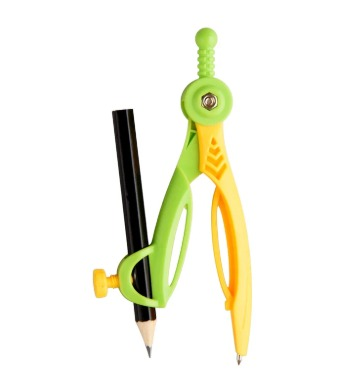
\includegraphics[width=0.4\textwidth]{compass_photo}
    \caption{Imagen de referencia de un compás escolar tradicional. Fuente: \cite{ref_img_compas}}
    \label{fig:ref_compas}
\end{figure}
\bigskip

\subsection{Articulaciones Mecánicas con Pasador}
Las articulaciones mecánicas con pasador son mecanismos fundamentales que permiten la conexión entre dos partes móviles, facilitando su rotación relativa, como se observa en el ejemplo de la Figura \ref{fig:ref_articulacion}. Se tomó como inspiración este tipo de mecanismo por su capacidad para ofrecer movimiento rotacional estable y controlado.
Según Shigley, Mischke y Budynas \cite{shigley_design}, \enquote{las articulaciones de pasador son ampliamente utilizadas en mecanismos para permitir la rotación con soporte y resistencia suficiente para mantener la posición sin movimientos no deseados} (p. 145). Esta característica es clave para resolver la rigidez del compás convencional.
\newpage

\begin{figure}[htbp]
    \centering
    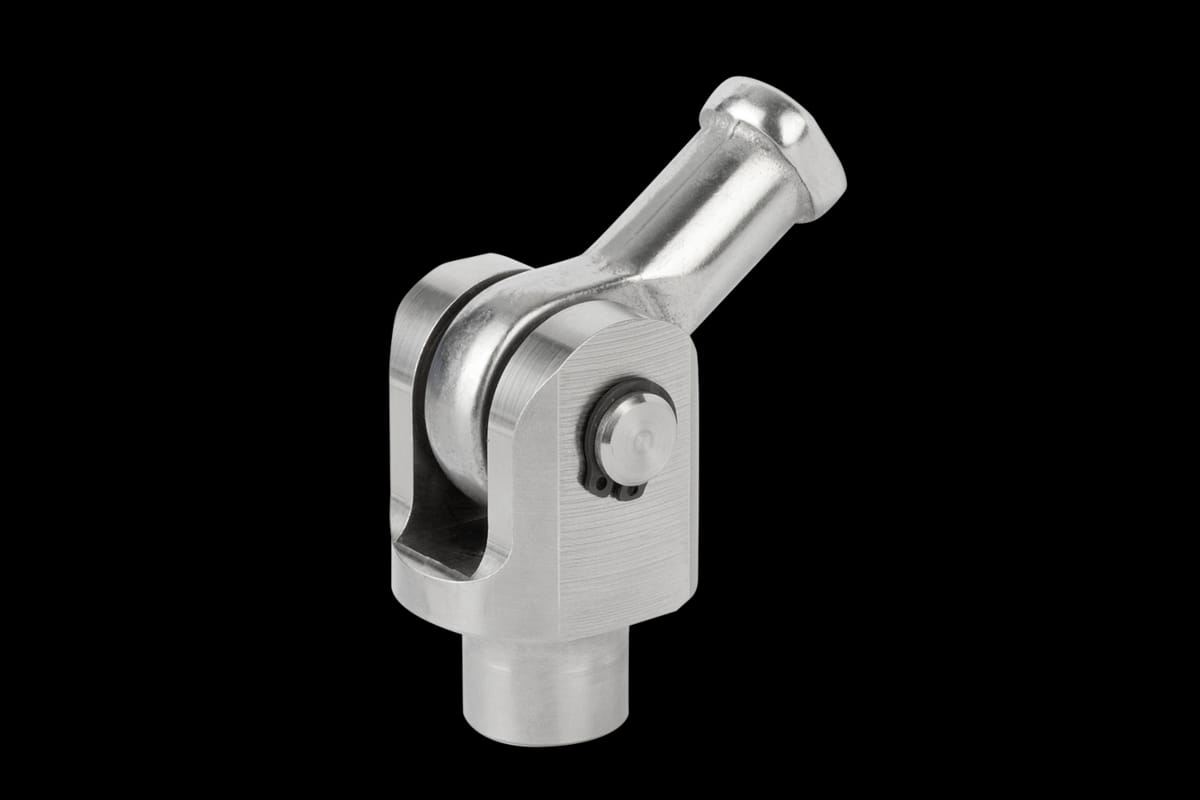
\includegraphics[width=0.5\textwidth]{articulacion_pasador}
    \caption{Ejemplo de referencia de una articulación de pasador tipo horquilla. Fuente: \cite{ref_img_articulacion}}
    \label{fig:ref_articulacion}
\end{figure}
\bigskip

\subsection{Justificación de la Elección}
En conjunto, estos mecanismos ofrecen una solución funcional y técnicamente viable, al combinar la precisión del compás clásico con la movilidad de las articulaciones de pasador. Esta fusión permite mejorar notablemente la experiencia del usuario, aportando comodidad, versatilidad y un mayor control sobre la expresión gráfica.
\bigskip


\section{Planificación del Proyecto (Carta Gantt)}
La distribución de tareas para la realización de este proyecto se detalla en la Tabla \ref{tab:gantt}.
\smallskip

\begin{table}[htbp]
    \centering
    \caption{Asignación y cronograma de actividades del proyecto.}
    \label{tab:gantt}
    \resizebox{\textwidth}{!}{%
    \begin{tabular}{@{}cllccc@{}}
        \toprule
        \textbf{Nº} & \textbf{Actividad} & \textbf{Duración} & \textbf{Día de inicio} & \textbf{Día de término} & \textbf{Responsable} \\
        \midrule
        1   & \textbf{Revisión del compás escolar original} & 2 días & Día 1 & Día 2 & Lucas Espinoza \\
        \cmidrule(l){2-2}
        1.1 & \hspace{1em}- Inspección visual & 1 día & Día 1 & Día 1 & Lucas Espinoza \\
        1.2 & \hspace{1em}- Pruebas de funcionalidad & 1 día & Día 2 & Día 2 & Lucas Espinoza \\
        \addlinespace
        2   & \textbf{Investigación técnica y bibliográfica} & 5 días & Día 3 & Día 7 & Lucas Espinoza \\
        \cmidrule(l){2-2}
        2.1 & \hspace{1em}- Búsqueda de fuentes & 2 días & Día 3 & Día 4 & Lucas Espinoza \\
        2.2 & \hspace{1em}- Análisis de mecanismos existentes & 2 días & Día 5 & Día 6 & Lucas Espinoza \\
        2.3 & \hspace{1em}- Documentación y resumen & 1 día & Día 7 & Día 7 & Lucas Espinoza \\
        \addlinespace
        3   & \textbf{Desarrollo de planos en AutoCAD} & 3 días & Día 8 & Día 10 & Lucas Espinoza \\
        \cmidrule(l){2-2}
        3.1 & \hspace{1em}- Bocetos preliminares & 1 día & Día 8 & Día 8 & Lucas Espinoza \\
        3.2 & \hspace{1em}- Modelado CAD & 2 días & Día 9 & Día 10 & Lucas Espinoza \\
        \addlinespace
        4   & \textbf{Redacción del informe final (PDF)} & 4 días & Día 11 & Día 14 & Lucas Espinoza \\
        \cmidrule(l){2-2}
        4.1 & \hspace{1em}- Organización de contenido & 1 día & Día 11 & Día 11 & Lucas Espinoza \\
        4.2 & \hspace{1em}- Redacción y edición & 2 días & Día 12 & Día 13 & Lucas Espinoza \\
        4.3 & \hspace{1em}- Revisión final y formato & 1 día & Día 14 & Día 14 & Lucas Espinoza \\
        \bottomrule
    \end{tabular}
    }
\end{table}
\newpage

\section{Desarrollo del Diseño}
\subsection{Boceto Inicial}
A partir de los mecanismos mencionados, se desarrolló el boceto del compás (Figura \ref{fig:boceto}). Este diseño conserva la ingeniería funcional del compás tradicional, pero introduce una modificación significativa en la zona de sujeción del lápiz, incorporando un mecanismo articulado.
Esta inclinación controlada ofrece múltiples ventajas: permite adaptar la herramienta a distintas formas de trazo, mejora la ergonomía y ofrece una mayor expresividad gráfica.

\begin{figure}[htbp]
    \centering
    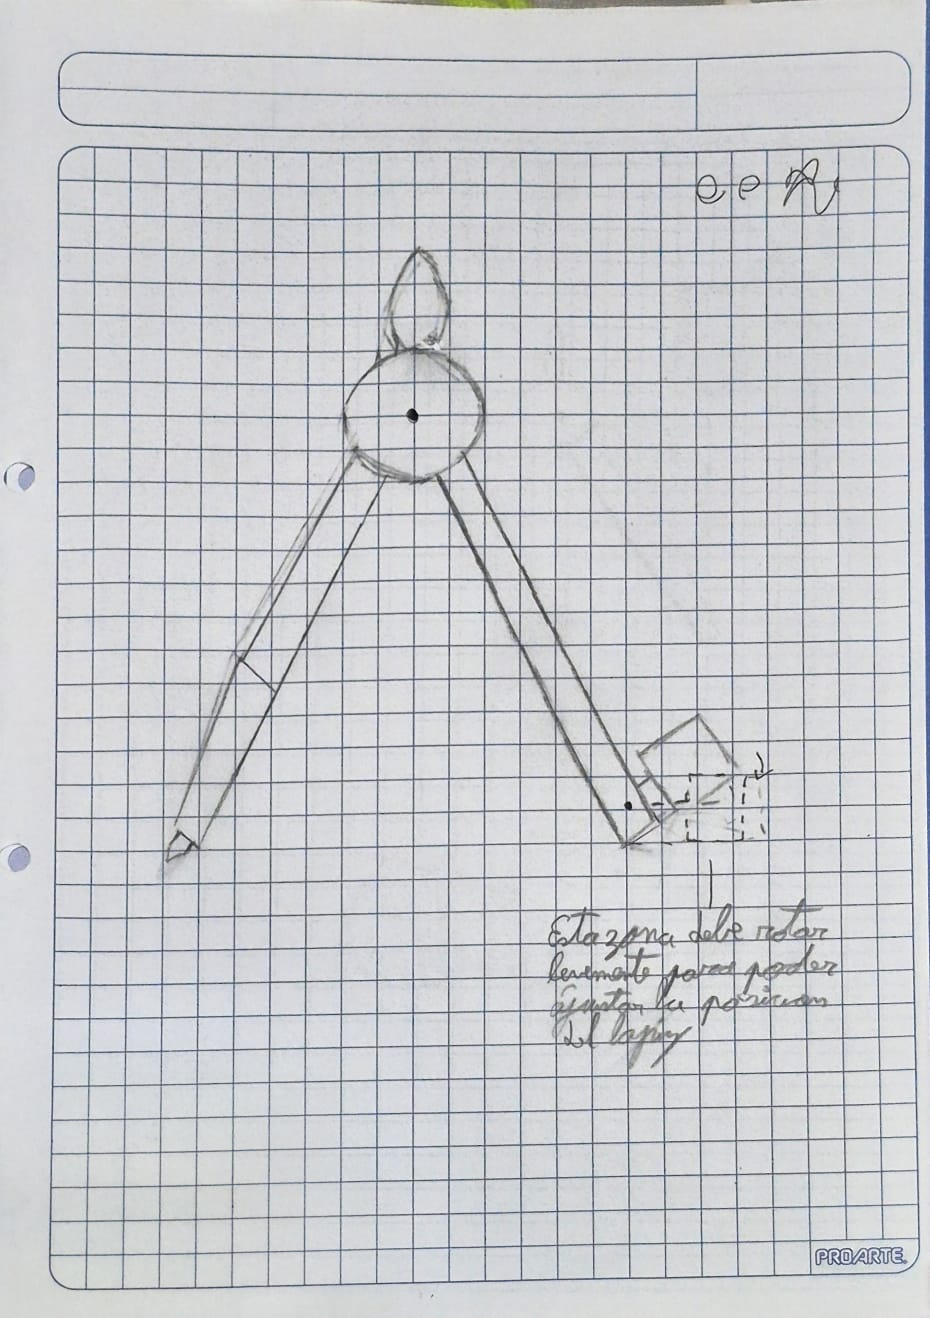
\includegraphics[width=0.7951\textwidth]{compass_sketch}
    \caption{Boceto inicial del compás mejorado. La nota manuscrita indica: "Esta zona debe rotar levemente para poder ajustar la posición del lápiz".}
    \label{fig:boceto}
\end{figure}
\newpage

\section{Resultados: Planos Técnicos}
En base al boceto y la propuesta de diseño, se han creado los planos técnicos del compás mejorado utilizando AutoCAD. Se incluyen el plano de conjunto, el plano de despiece y los planos de fabricación.

\subsection{Plano de Conjunto}
La Figura \ref{fig:conjunto} muestra el ensamblaje completo del compás, identificando cada componente con su respectivo número de marca y la lista de piezas.

\begin{figure}[htbp]
    \centering
    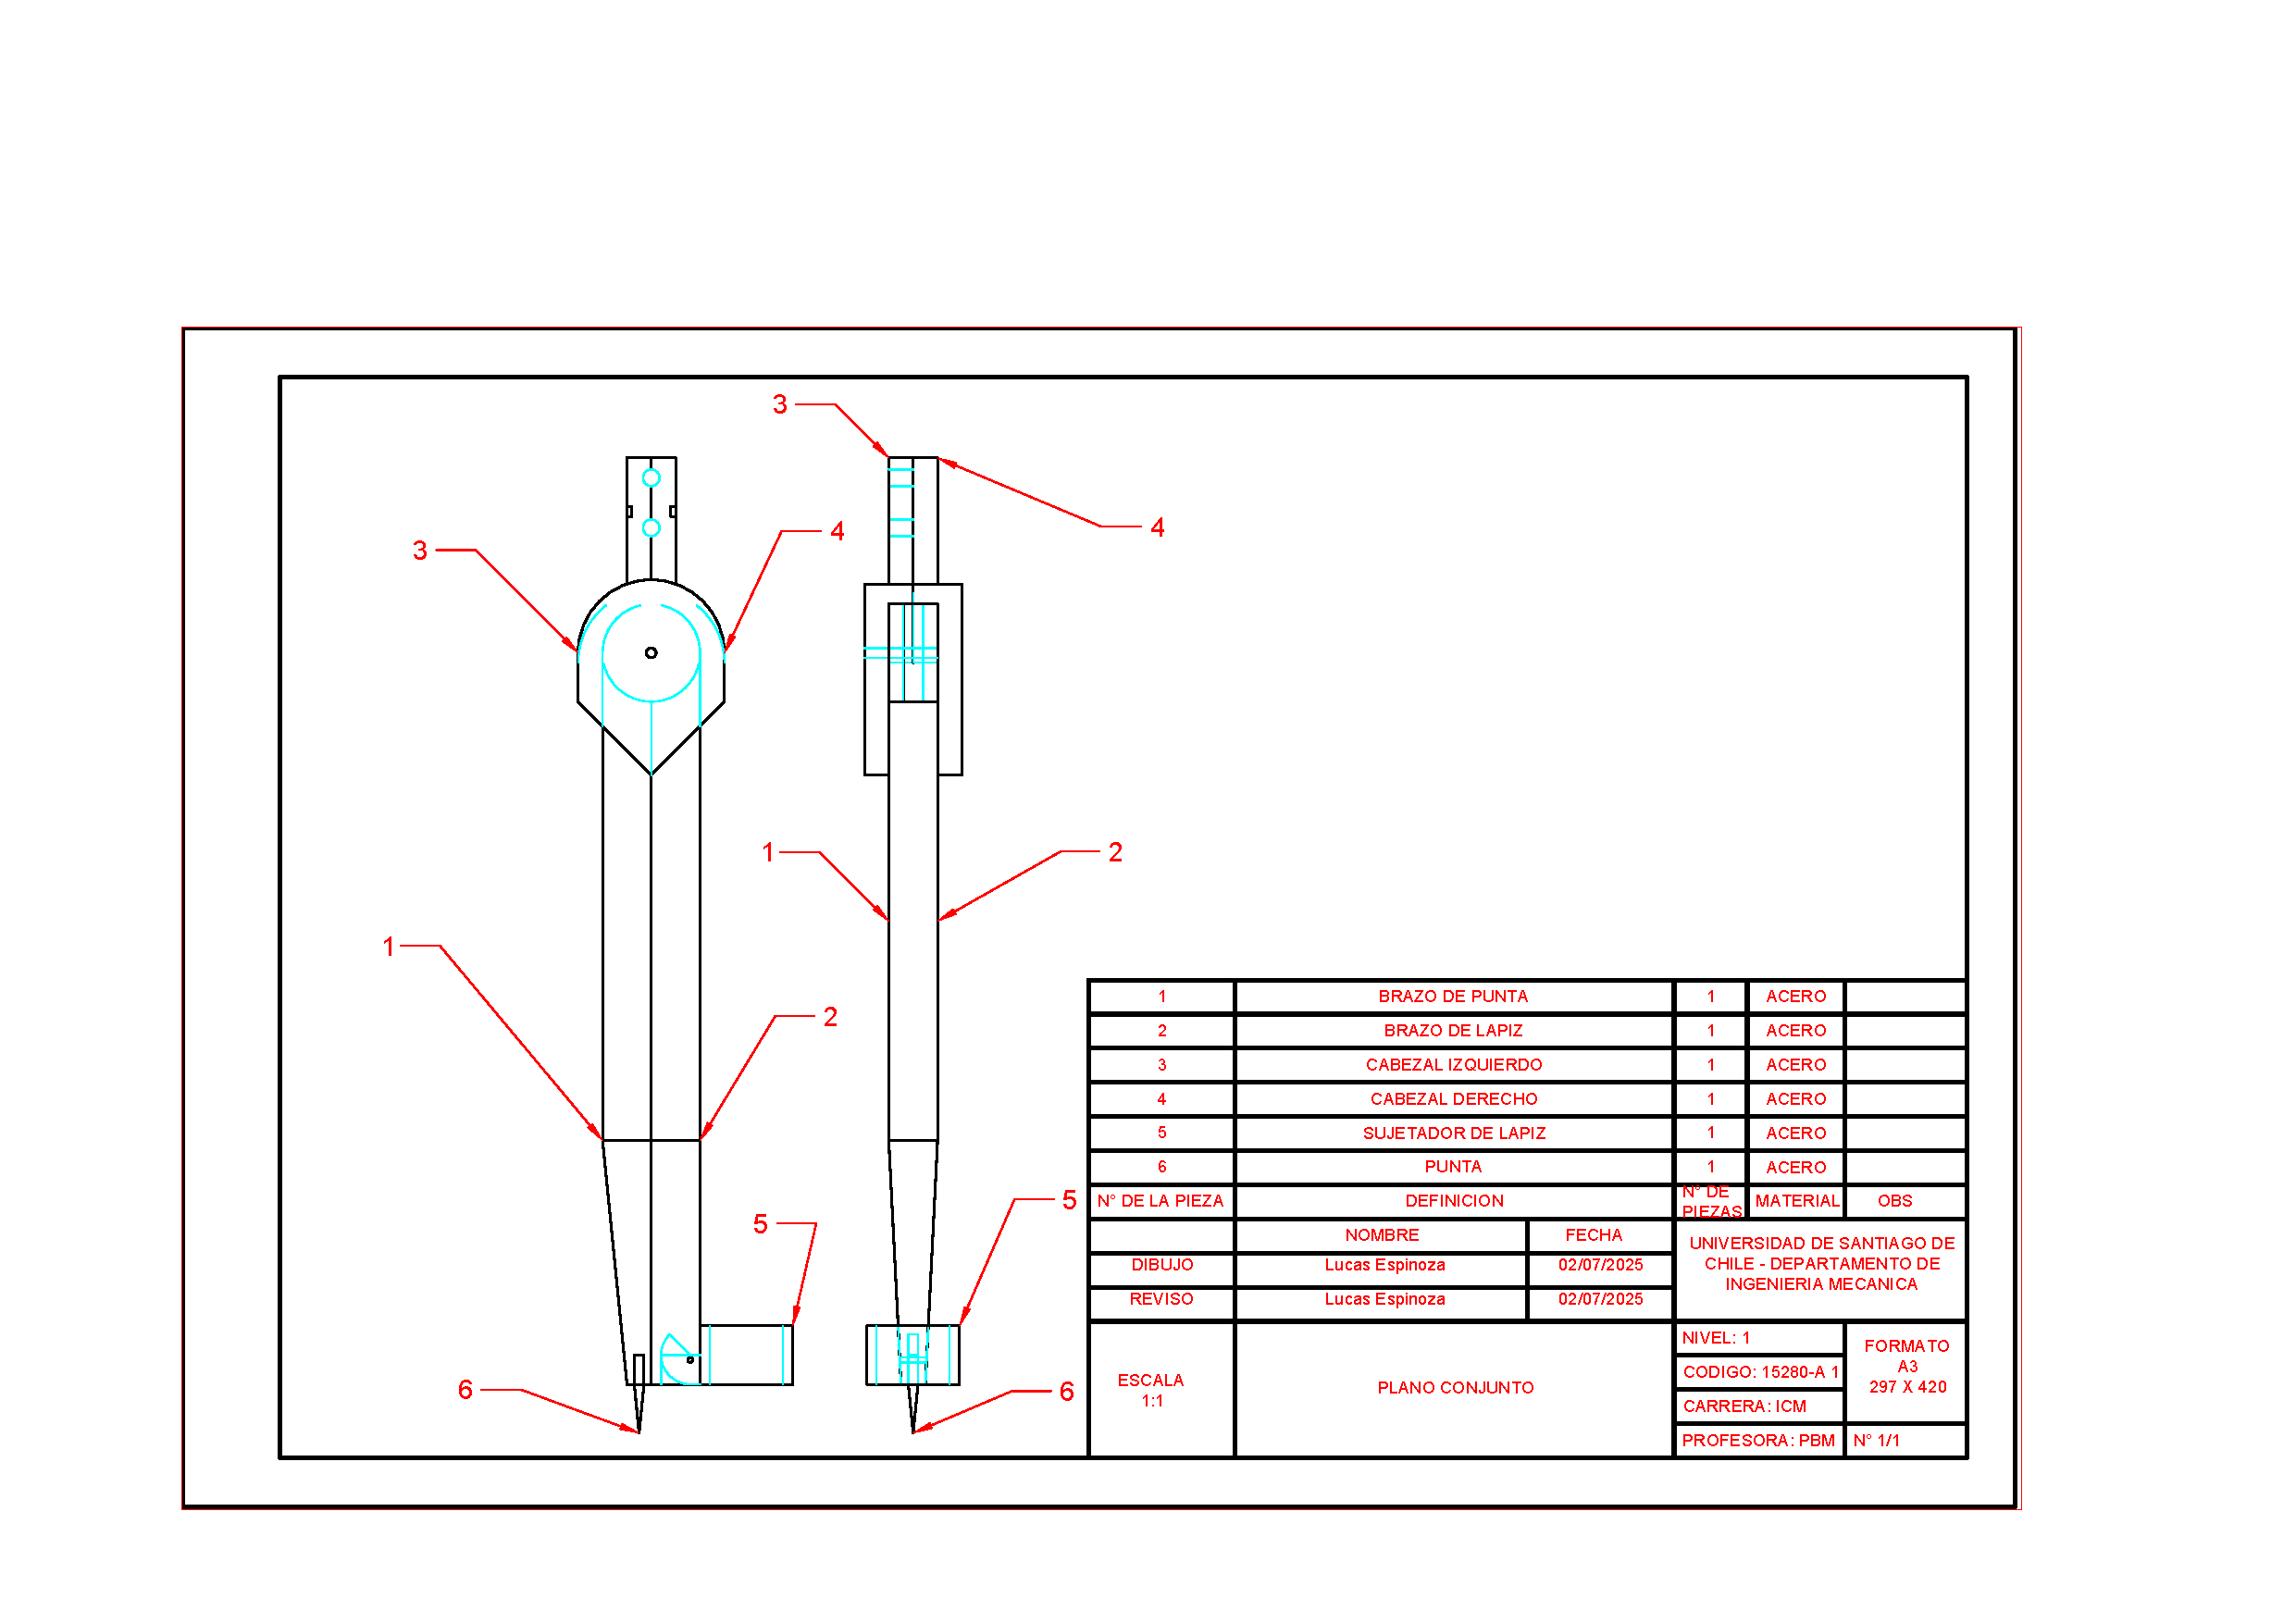
\includegraphics[width=\textwidth, keepaspectratio]{plano_conjunto}
    \caption{Plano de conjunto del compás de trazado mejorado.}
    \label{fig:conjunto}
\end{figure}
\newpage

\subsection{Plano de Despiece}
El plano de despiece (Figura \ref{fig:despiece}) presenta una vista detallada de cada una de las 6 piezas que conforman el mecanismo, con sus acotaciones principales.

\begin{figure}[htbp]
    \centering
    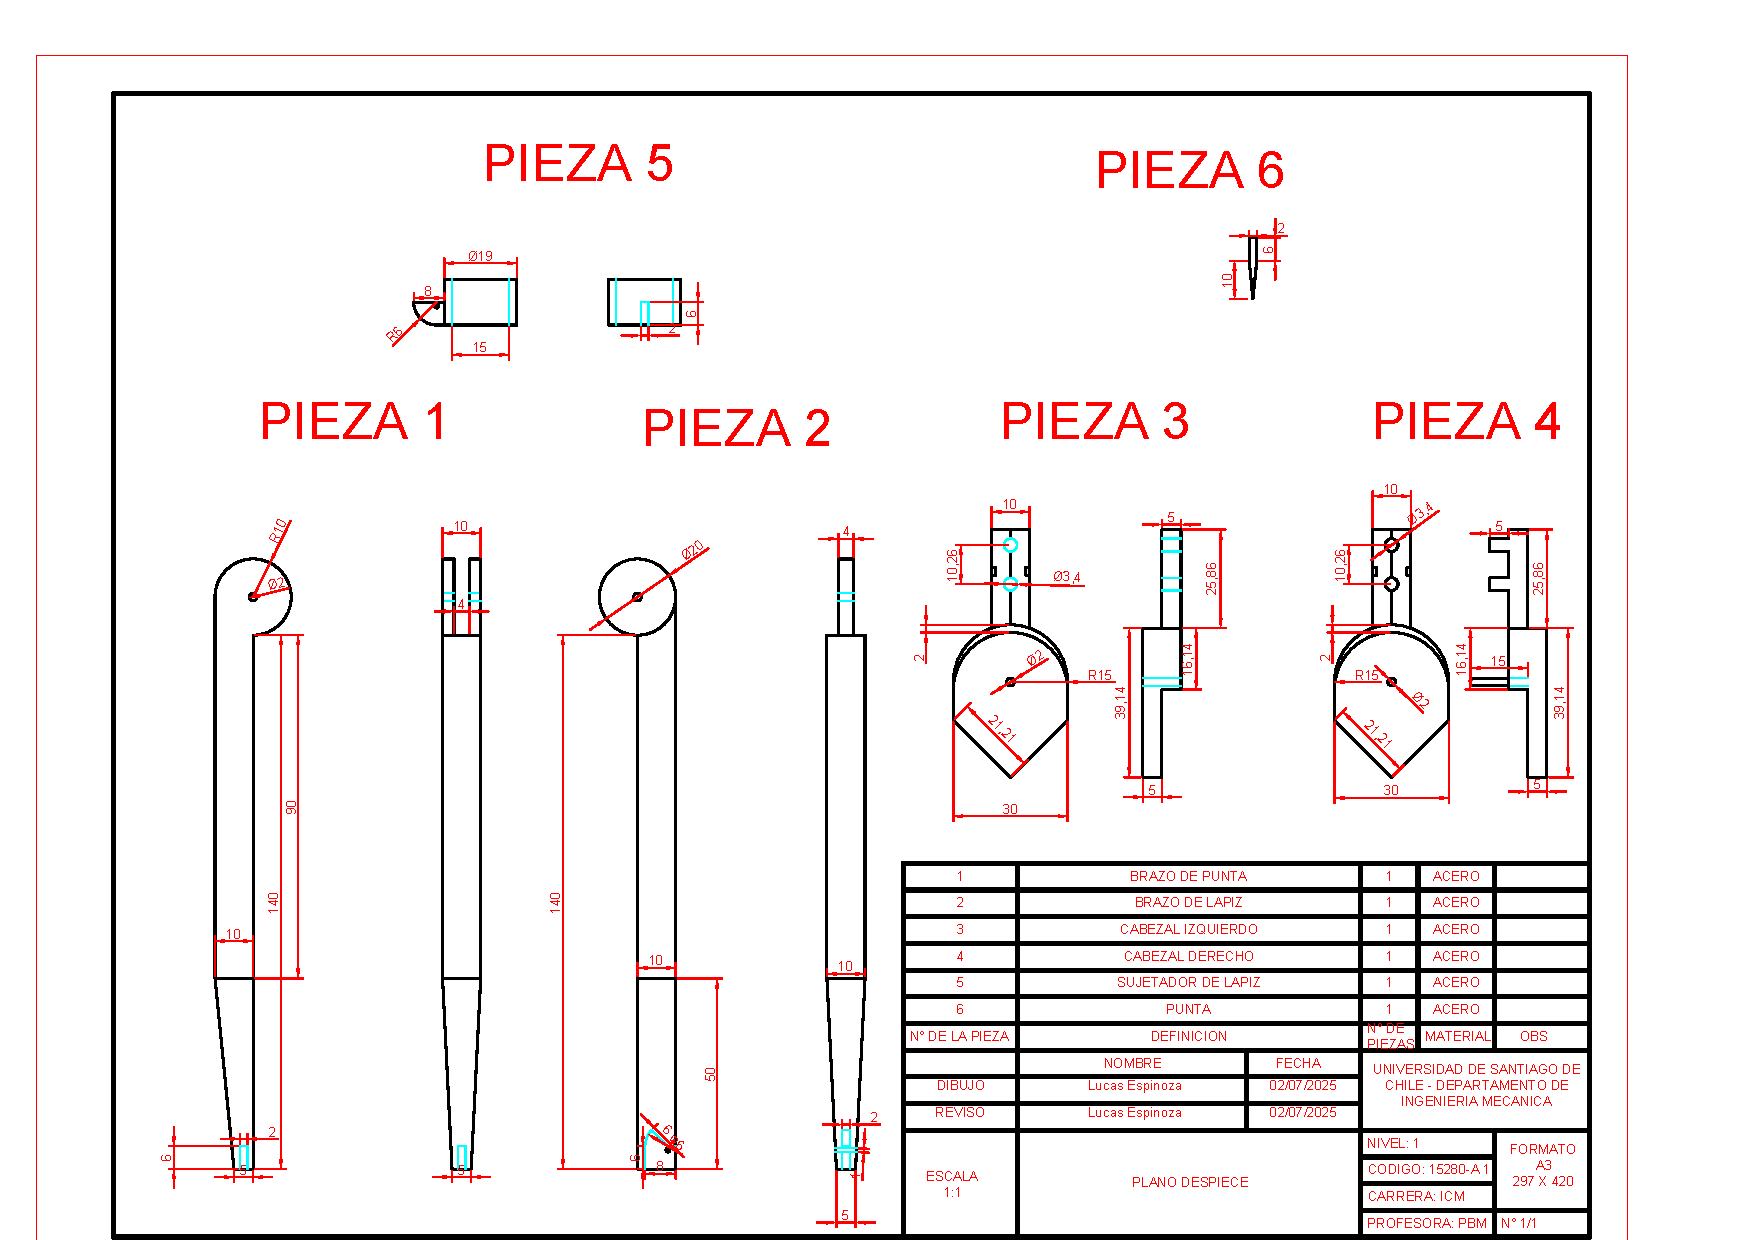
\includegraphics[width=\textwidth, keepaspectratio]{plano_despiece}
    \caption{Plano de despiece del compás, mostrando las 6 piezas diseñadas.}
    \label{fig:despiece}
\end{figure}
\newpage

\subsection{Planos de Fabricación}
La Figura \ref{fig:fabricacion} muestra los planos de fabricación individuales para cada una de las piezas diseñadas. Cada plano contiene las vistas y cotas necesarias para su manufactura.

\begin{figure}[htbp]
    \centering
    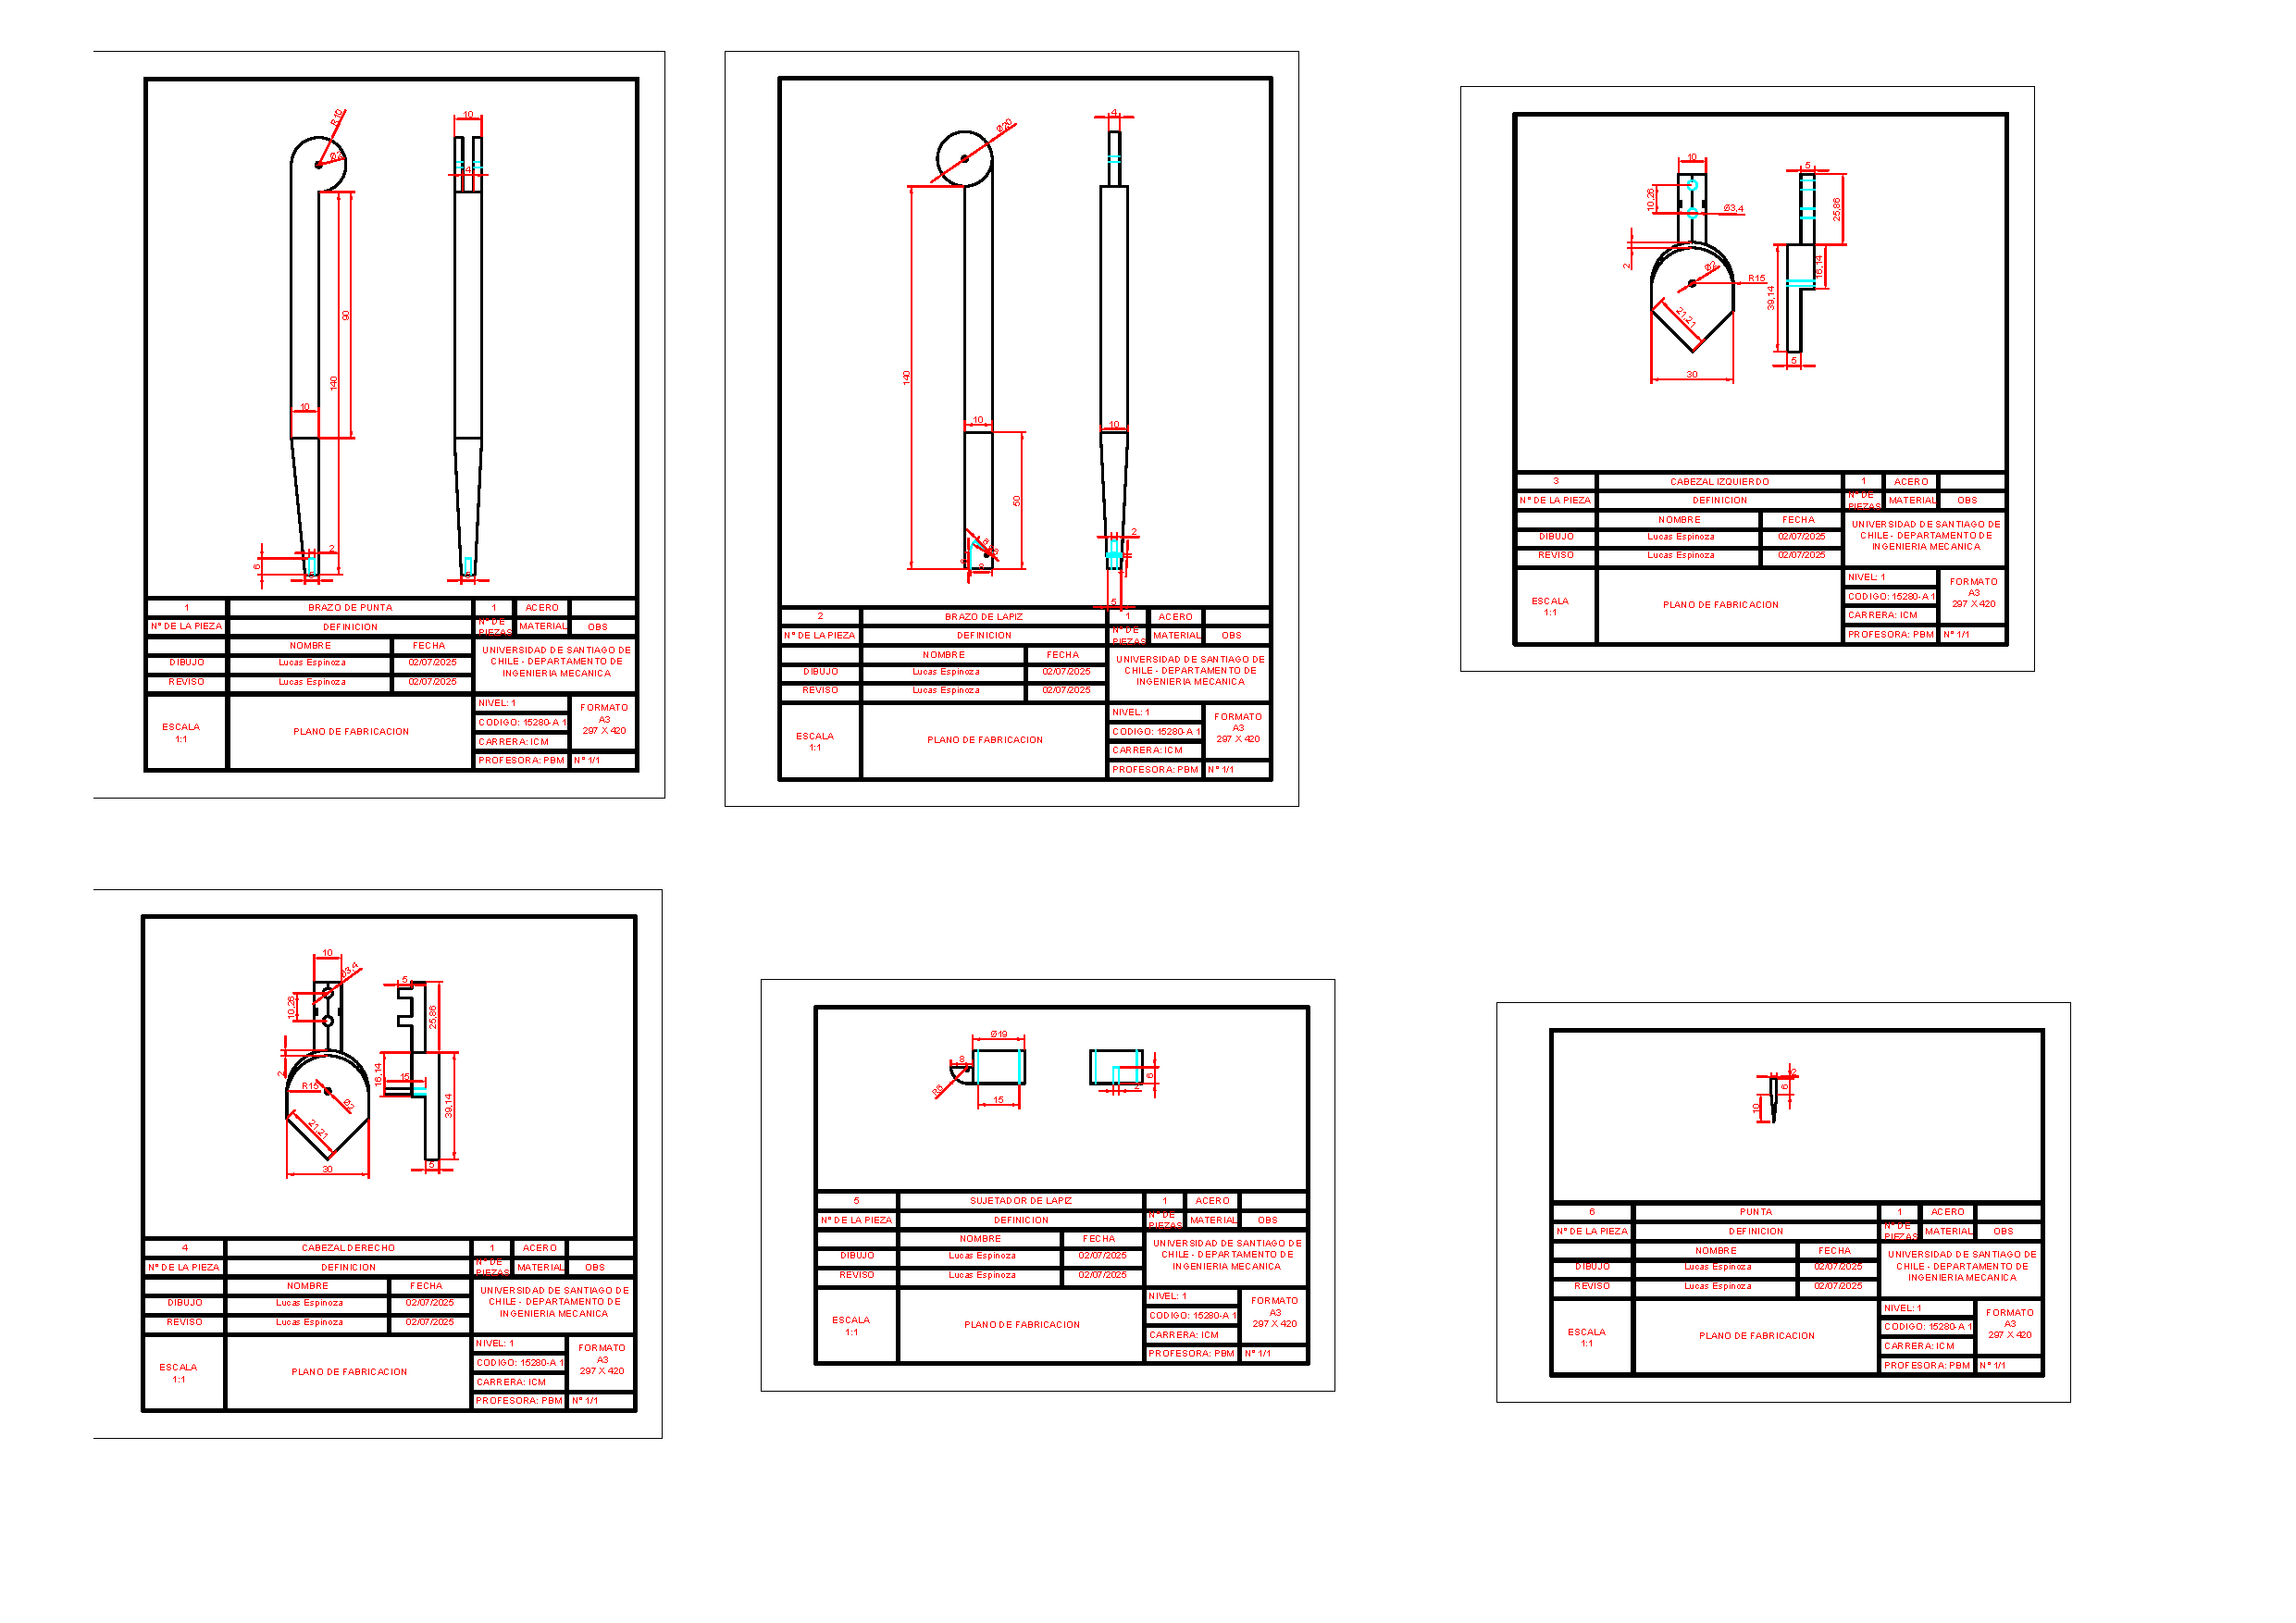
\includegraphics[width=\textwidth, keepaspectratio]{planos_fabricacion}
    \caption{Planos de fabricación para las 6 piezas del compás.}
    \label{fig:fabricacion}
\end{figure}

\newpage
\section{Conclusiones}
El proyecto de diseño y mejora de un compás escolar ha culminado exitosamente en una propuesta que resuelve de manera efectiva la principal limitación de los modelos tradicionales. La incorporación de un mecanismo articulado en el brazo porta-lápiz otorga al usuario un grado de libertad adicional, permitiendo la inclinación del trazo sin sacrificar la estabilidad y precisión del instrumento.

El análisis de mecanismos de referencia fue fundamental para concebir una solución viable, combinando la simplicidad estructural del compás clásico con la funcionalidad de una articulación de pasador. El proceso de diseño, documentado desde el boceto inicial hasta los planos técnicos finales, demuestra la factibilidad de la propuesta. Los planos de conjunto, despiece y fabricación, elaborados en AutoCAD bajo la normativa chilena, constituyen una guía completa para la eventual construcción de un prototipo.

Finalmente, este proyecto no solo representa una solución a un problema técnico, sino que también pone en práctica los conocimientos de dibujo de ingeniería, planificación y documentación de proyectos, cumpliendo con todos los objetivos planteados en la asignatura.

\printbibliography[title={Bibliografía}]

\end{document}
